% $Id: pkg-example.tex,v 1.9 2003/10/01 21:27:46 naughtont Exp $

\section{Example Package}
\label{sect:example-pkg}

\subsection{A basic \file{config.xml}}
\label{sect:example-config-xml}

The following shows the meta file for a package called SSSlib.  

\begin{verse}
   {\bfseries Notice: } Due to the XML parser module used, currently
   multi-line elements like \xmltag{description} must have the closing tag
   on the same line as the last line of text.  
\end{verse}


\begin{scriptsize}
\begin{verbatim}
<?xml version="1.0" encoding="ISO-8859-1"?>
<oscar>
  <name>SSSLib</name>

  <version>
    <major>0</major>
    <minor>95</minor>
    <subversion>2</subversion>
    <release>1</release>
    <epoch>1</epoch>
  </version>

  <class>third-party</class>
  <installable>1</installable>

  <summary>SciDAC:SSS Infrastructure components</summary>
  <license>GPL</license>
  <group>Application/System</group>
  <url>http://www.scidac.org/ScalableSystems</url>
  
  <maintainer>
     <name>Narayan Desai</name>
     <email>narayan@anl.gov</email>
  </maintainer>

  <packager>
    <name>Thomas Naughton</name>
    <email>naughtont@ornl.gov</email>
  </packager>

  <description>The BCWG Infrastructure components for the SciDAC: Scalable 
Systems Software.  These infrastructure components include the Service 
Directory, Event Manager, etc. as well as the communication 
library. </description>

  <rpmlist>
        <filter distribution="redhat" distribution_version="7.2" architecture="ia32"/>
        <filter distribution="mandrake" distribution_version="8.2"/>
        <rpm>ssslib</rpm>
        <rpm>sss-clients</rpm>
        <rpm>sss-infrastructure</rpm>
        <rpm>ssslib-perl</rpm>
        <rpm>ssslib-python</rpm>
        <rpm>sss-nsm-client</rpm>
        <rpm>sss-old</rpm>
        <rpm>sss-schemas</rpm>
        <rpm>sss-validate</rpm>
        <rpm>sss-validate-python</rpm>
	</rpmlist>

	<rpmlist>
        <filter group="oscar_server" distribution="redhat" distribution_version="7.2"/>
        <filter group="oscar_server" distribution="redhat" distribution_version="7.3"/>
        <rpm>sss-mayor-slave</rpm>
        <rpm>sss-servers</rpm>
  </rpmlist>
</oscar>
\end{verbatim}
\end{scriptsize}


\subsection{Using the Configurator}
\label{sect:example-configurator}

The following is an example \file{configurator.html} used to setup a
configuration file.  Default values are seeded so a user can simply click
``Ok'' if they like.

\begin{scriptsize}
\begin{verbatim}
<html>
  <head> 
    <title>SSSLib Configuration Settings</title> 
  </head> 

  <body>
    <form>
    <center>
    <h2>Setup SSSLib Configuration File</H2>
    </center>
    <br>

    <p> Hostname where Service Directory runs<br>
    <input name="sd_host" value="oscar_server"><br>

    <p> Port number for Service Directory<br>
    <input name="sd_port" value="7000"><br>

    <p> Default protocol for Service Directory<br>
    <select name="sd_protocol" size=1>
    <option selected>challenge
    <option>basic
    </select><br>

    <p> Preference ordering for protocols<br>
    <input name="prefs" value="challenge,basic"><br>

    <p> Cluster name<br>
    <input name="cluster" value="oscar_cluster"><br>

    <p> Challenge protocol password<br>
    (Currently stored in plain text)<br>
    <input name="password" value="OscarSSSpass"><br>   

    <p> <input type="checkbox" name="msg_log" value="/var/log/sss_msg.log">
    Enable message logging (logfile='/var/log/sss_msg.log')<br>

    <p> <input type="checkbox" name="syslog_sss" value="/var/log/sss.log">   
    Enable additional logging via syslog (logfile='/var/log/sss.log')<br>

    <p> <input type="reset" value='Reset Form'>
    </form>
  </body> 
</html>
\end{verbatim}
\end{scriptsize}

Below is an image of this HTML code as rendered by the Configurator:

\begin{quote}
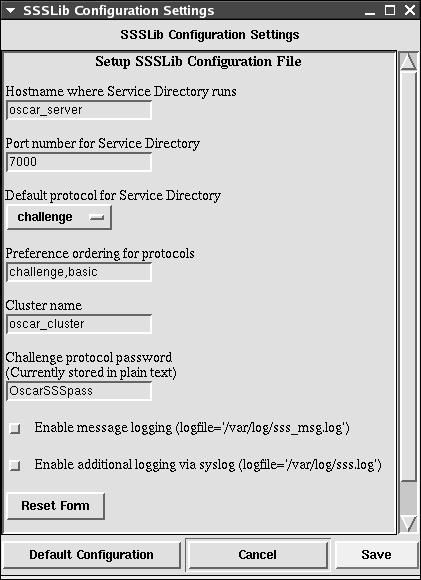
\includegraphics[scale=0.3]{figs/ConfiguratorExample}
\end{quote}



\subsubsection{post\_configure}

This is a simple \file{post\_configure} example that process the results
of the Configurator that are stored in the XML \file{.configurator.values}
file.  This reads those values to generate a configuration file
\file{/etc/ssslib.conf}.

\begin{scriptsize}
\begin{verbatim}
  #!/usr/bin/env perl
  # 'post_configure' -- reads Configurator result to setup '/etc/ssslib.conf'

  use XML::Simple;
  use Carp;

  my @fields = (sd_host, sd_port, sd_protocol, prefs, cluster, password, 
                msg_log, syslog_sss);
  my $conf     = ">/etc/ssslib.conf";
  my $xml_data = "$ENV{OSCAR_PACKAGE_HOME}/.configurator.values";


  my $ref = XMLin($xml_data) or croak("Error: unable to open ($xml_data)");
  open(CONF, $conf) or croak("Error: unable to open ($conf)\n");

  print CONF "# SSSLib configuration file\n# Generated by OSCAR\n\n";
  foreach $key  (@fields) {
          if( defined($ref->{"$key"}) ) {
                  print CONF $key, "=", $ref->{$key}, "\n";
          }
  }
  print CONF "\n";

  close(CONF);
\end{verbatim}
\end{scriptsize}

There is one important issue with multiline $<$select$>$ elements.  If the
user selects only one $<$option$>$, XMLin() in its basic form above will
return the value for the $<$select$>$ element as a SCALAR.  But if the user
selects multiple $<$option$>$s, XMLin() will return the value as an ARRAY.
To handle this case you have two options:

\begin{enumerate}
\item Use the Perl function \texttt{ref()} to determine if each hash value is
an ARRAY or a SCALAR and handle it appropriately.  
\item Call XMLin as \texttt{XMLin(FILENAME, forcearray => '1')}.  This will
force every hash value to be an array.  Thus, you can either iterate through
all hash values, or you can access the 0th element of the hash value for
those inputs you know will have only one value.
\end{enumerate}



% TJN: Finish this section...
\subsection{post\_clients}

This is an example taken from C3 that builds the \file{/etc/c3.conf} using
the information that was obtained after the nodes of the cluster have been
defined. 
\begin{scriptsize}
\begin{verbatim}
#!/usr/bin/perl
# 'post_clients' -- generate the C3 configuration file '/etc/c3.conf'

use strict;
use Carp;
use lib '/usr/lib/systeminstaller';
use SystemInstaller::Machine;
use Data::Dumper;

my $image = shift;

my $c3_conf = "/etc/c3.conf";

my $hostname = `hostname`;
chomp($hostname);

my %hash = get_machine_listing($image);

open(OUT,">$c3_conf") or croak("Couldn't open $c3_conf");
print OUT "cluster oscar_cluster {\n";
print OUT "\t$hostname\n";
my $firstkey = 1;
foreach my $key (sort numerically keys %hash) {
    if ($firstkey)
      {
        $hash{$key}->{HOST} =~ /([a-zA-Z_\-]+)(\d*)/;
        print OUT "\tdead remove_line_for_0-indexing\n" if 
          (defined($2) && ($2 != 0));
        $firstkey = 0;
      }
    print OUT "\t", $hash{$key}->{HOST}, "\n";
}
print OUT "}\n";
close(OUT);



# Sort hostnames numerically instead of an ascii sort.
# Special sort() sub-rtn (uses $a, $b instead of @_)
sub numerically
{
    $a =~ /(\d+)$/;  # pickoff number and
    my $A = $1;      #  save in local var

    $b =~ /(\d+)$/;  # pickoff number and
    my $B = $1;      #  save in local var

    ($A <=> $B)
}
\end{verbatim}
\end{scriptsize}


\subsection{post\_install}

These two examples show two very simple examples of OSCAR packages that are
using this final phase script.  The OPIUM package is used to synchronize
system files across the cluster, e.g., account files like '/etc/passwd',
etc.  It takes a simple option to \cmd{--force} synchronization once all
nodes have been built since the account information is not stored in the
image that is used to build the machines.

\begin{scriptsize}
\begin{verbatim}
    #!/bin/sh
    /opt/opium/bin/sync_users --force
\end{verbatim}
\end{scriptsize}


\noindent The other package example making use of \file{post\_install} is the
NTP configuration package.  It uses a C3 parallel execution command to
restart the NTP daemon on all nodes of the cluster.

\begin{scriptsize}
\begin{verbatim}
    #!/bin/bash
    # Post install action to restart ntpds.  This is necessary because when the
    # node is booting for the first time, other nodes are sometimes building,
    # causing network saturation.  This causes the ntpd to give up and try
    # later.
  
    . /etc/profile
    cexec /etc/init.d/ntpd restart
\end{verbatim}
\end{scriptsize}
